\chapter{A Reinforcement Learning Approach to Black-Box Optimization}

One of the principal challenges in optimization practice is how to optimize in absence of an algebraic model of the system to be optimized. This kind of optimization is known as \textit{black-box optimization}. \\

A black-box function $f(x) : \mathbb{R}^n \rightarrow \mathbb{R}$ is a function for which the analytic form is not known. Nowadays there are lots of mathematical models to solve these type of functions. One of the best known of these methods is the \textit{Bayesian Optimization Model} (BO). \\
In this chapter we will first explain how BO works and than we will propose an innovative, RL based approach for black-box optimization problem.

\paragraph{Gaussian Processes} Before starting to speak about BO we have to describe what \textit{Gaussian Processes} (GPs) are. GPs are an alternative approach to regression problems. The GP approach is a \textit{non-parametric} (we don't have a priori knowledge of how many parameters will be useful for our regression) approach to find a distribution over the possible function $f(x)$ that are consistent with observed data. A GP is a generalization of the Gaussian probability distribution. Whereas a probability distribution describes random variables which are scalars or vectors (for multivariate distributions), a stochastic process governs the properties of functions.
GP is a convenient and powerful prior distribution on functions, which we will take here to be of the form $f : \mathcal{X} \leftarrow \mathbb{R}$. The GP is defined by the property that any finite set of $N$ points $\{x_n \in \mathcal{X}\}\subsup{}{ n=1}{N}$ induces a multivariate Gaussian distribution  on $\mathbb{R}^N$. The $n$th of these points is taken to be the function value $f(x_n)$. The support and properties of the resulting distribution on functions are determined by a mean function $m : \mathcal{X} \leftarrow \mathbb{R}$ and a positive definite covariance function $K : \mathcal{X} \times \mathcal{X} \leftarrow \mathbb{R}$ ~\cite{NIPS2012_4522}.

\begin{figure} [h!]
	\centering
	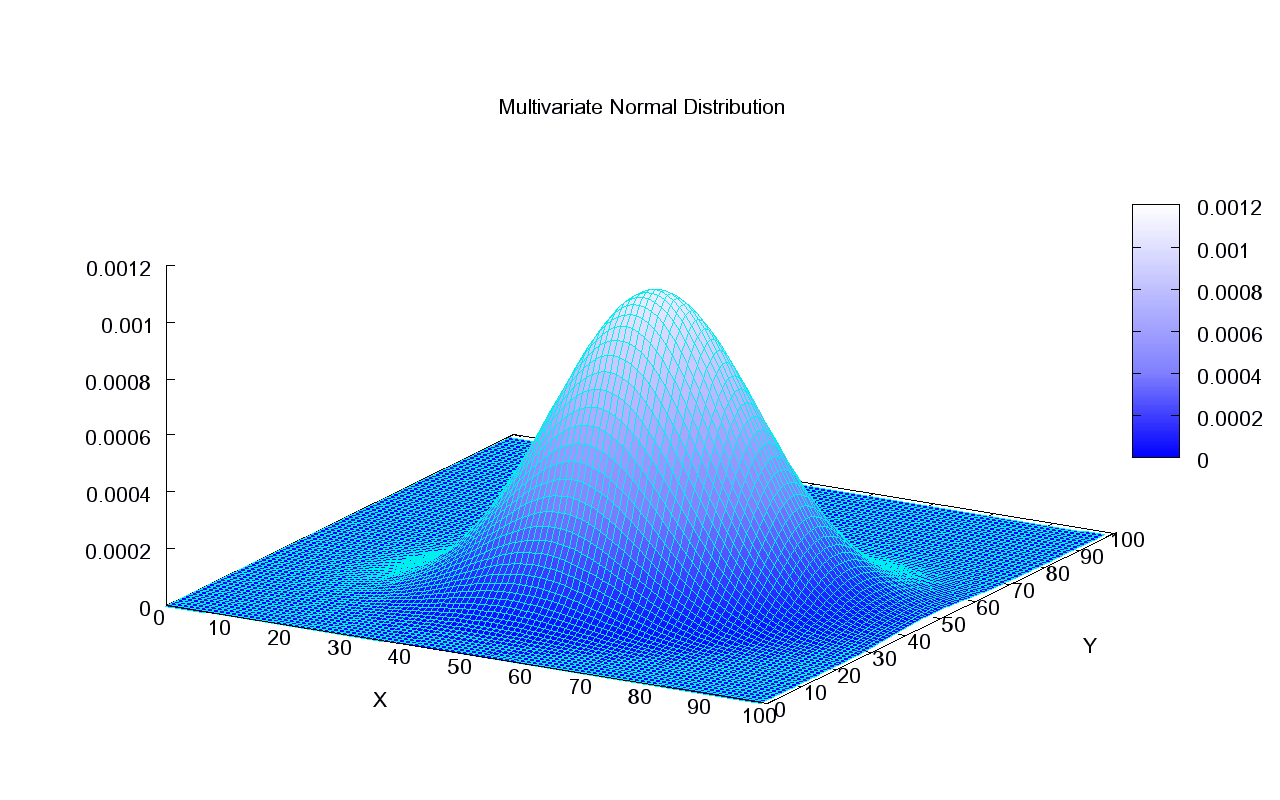
\includegraphics[width= \textwidth, height = 9.5cm]{Multivariate_Gaussian.png}
	\caption{Multivariate Gaussian Distribution [Wikipedia]}
	\label{fig:Multivatiate_Gaussian}
\end{figure}

\paragraph{Acquisition Functions for Bayesian Optimization} Let's assume that the function $f(x)$ is drawn from a GP prior and that our observation are of the form $\{x_n \in \mathcal{X}\}\subsup{}{ n=1}{N}$, where $y_n \sim \mathcal{N}(f(x_n), v)$ and $v$ is the variance of noise introduced into the function observations. This prior and these data induce  posterior over functions; the acquisition function, which we denote by $a : \mathcal{X} \leftarrow \mathbb{R}^+$, determines what point in $\mathcal{X}$ should be evaluated next via a proxy optimization $x\textsubscript{next} = \arg\max_{x}a(x)$, where several different functions have been proposed. There are several popular choices of acquisition function. Under the Gaussian process prior, these functions depend on the model solely through its predictive mean function $\mu(x; \{x_n, y_n\})$ and predictive variance function $\sigma^2(x; \{x_n, y_n\})$~\cite{NIPS2012_4522}.

\begin{figure} [h!]
	\centering
	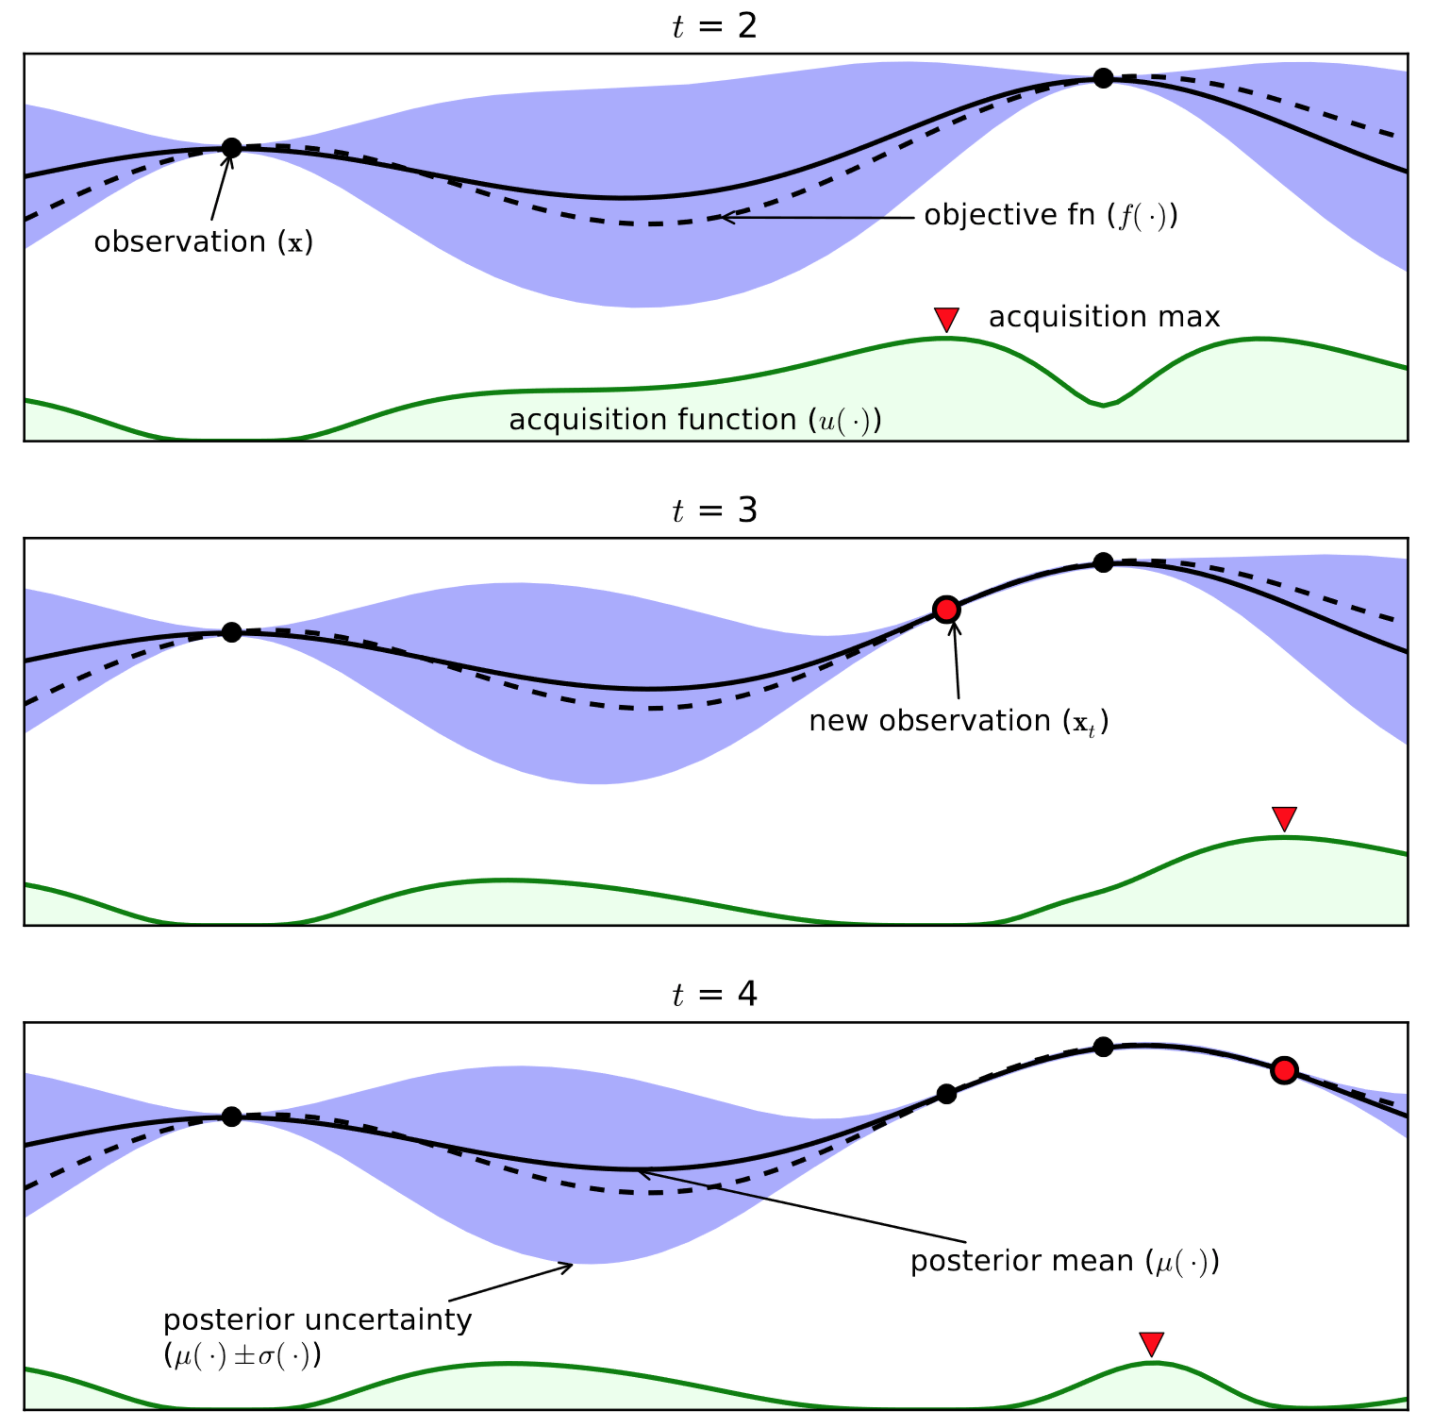
\includegraphics[width= \textwidth, height = 13cm]{BOProcess.png}
	\caption{2-$d$ Bayesian Optimization Process Example[towardsdatascience.com]}
	\label{fig:BoProcess}
\end{figure}